\documentclass[12pt,a4paper]{report}
\usepackage[pdftex]{graphicx}  % compiled by pdftex
\usepackage{graphicx}
\usepackage[margin=2.0cm]{geometry} % control margin of page
\usepackage{url}
\usepackage[center]{caption2}
\usepackage[colorlinks,linkcolor=blue,anchorcolor=blue,citecolor=green]{hyperref} % hyper reference to contents 
% \usepackage[bf,small,center,indentafter,pagestyles]{titlesec} % change section title
\parskip=3mm
\newcommand{\opal}{\textsc{OPAL }}
\newcommand{\opalt}{\textsc{OPAL-t }}
\newcommand{\opalcycl}{\textsc{OPAL-cycl }}
\newcommand{\opalmap}{\textsc{OPAL-map }}
\newcommand{\rnb}{radially neighboring bunches }
\newcommand{\sce}{Space charge effects }
\newcommand{\scf}{Space charge force }
\newcommand{\bs}[1]{\mathbf #1}
\newcommand{\HRule}{\rule{\linewidth}{0.5mm}}

\begin{document}

  %%%%%%%%%%%%%
  \begin{titlepage}
    
    \begin{center}
    
            
      %\textsc{\LARGE Internal Report}\\[1.5cm]
      
      \textsc{\Large Internal Report}\\[5.0cm]
  
      % Title
      \HRule \\[0.4cm]
	     { \huge \bfseries Modeling of 450 MeV Carbon Cyclotron}\\[0.4cm]
	     
     \HRule \\[1.5cm]
	
     \emph{Author:}\\[0.7cm]
     Jianjun \textsc{Yang}, 
     Andreas \textsc{Adelmann}\\ 
     \emph{AMAS Group, Paul Scherrer Institute, Switzerland}\\ [1.0cm]
          
     \vfill
     
     % Bottom of the page
	 {\large \today}
	 
    \end{center}
    
  \end{titlepage}
  %%%%%%%%%%%%
PSI is planing to build a new superconducting seperate-sector cyclotron for therapy purperse, which will accelerates the injected 250MeV/N Carbon(A=12.0, Z=6) 
particles to 450MeV/N at the extraction point. Mr. Joho and Negrazus give priliminay layout of the sectors structure and the shape of the sectors. 
The RF frequency is 100MHz and harmonic number is 12. the magnetic field at sector regin is homogeneous and its value is 4.0 Tesla.  The inner radius of sector 
is 3.3m and outer radius is 4.5m.

To obtain the basical facusing characteristic of the magnetic field, \opalcycl  is firstly used to caculate the betatron oslication frequency, namely, betatron tune. 
To do this, a small code is developed to generate the fild map on median plan. As the fridge fields of two side edges is very important for facusing characteristic, 
especally on virtical direction, the Enge's empirical function (NIM A 540 (2005) 1-13) is used as an approach of fridge fields.
\begin{equation}
  \label{eq:fridgefiled}
  B_z(x,0)= B_{max}h(x) = B_{max}\frac{1}{1+exp(c_0 + c_1 x + c_2 x^2 + c_3 x^3 + c_4 x^4 + c_5 x^5)}
\end{equation}
In our case, $x$ is the azimuthal distance to the hard edge of magnet in units of the full gap of the sector magnet. 
$c_0=-0.4785, c_1=2.9215, c_2=-0.8683, c_3=0.2000, c_4=-0.0300, c_5=0.0020$
\begin{figure}[ht]
  \begin{center} 
    {\includegraphics[width=10cm]{fringeCurve.pdf}}
    \caption{the generated field along azimuthal angle of Carbon Cyclotron}
    \label{fig:fielcurve}
  \end{center}
\end{figure}
Because 6 sectors are totally equal and the field is repeated after each 60 degree, only 1/6 field data is generated by the code and stored in memory when run \opalcycl.
For more detail of the setting for tuning calculation, one can refer to the OPAL User Guide.

Betatron tune is calculated from 250 MeV to 450 MeV after each 20 MeV. Firstly, run single particle tracking of \opalcycl to scan the approximately matched initial 
conditions for each energy. Then run tune calculation mode of \opalcycl. Figure\ref{fig:carbontune} shows the tune result and Figure\ref{fig:carbonorbit} shows 
the closed orbit result.   
\begin{figure}[ht]
%  \begin{minipage}[t]{0.3\textwidth}
    \centering 
	{\includegraphics[width=13cm]{tune.pdf}}
	\caption{Tune of carbon cyclotron}
	\label{fig:carbontune}
\end{figure}
\begin{figure}[ht]
%  \end{minipage}  
 % \begin{minipage}[t]{0.3\textwidth}
    \centering
	%{\includegraphics[width=10cm]{figures/Carbon/ClosedOrbit.pdf}}
	\rotatebox{-90}{\includegraphics[width=10cm]{ClosedOrbit.png}}
	\caption{Closed orbit of the mininal and maximal energy}
	\label{fig:carbonorbit}
  %\end{minipage}  
\end{figure}

\end{document}



